\documentclass{article}
\usepackage{tikz}
\usetikzlibrary{automata, positioning, arrows.meta}
\usepackage{pdflscape}

\begin{document}
\begin{landscape}
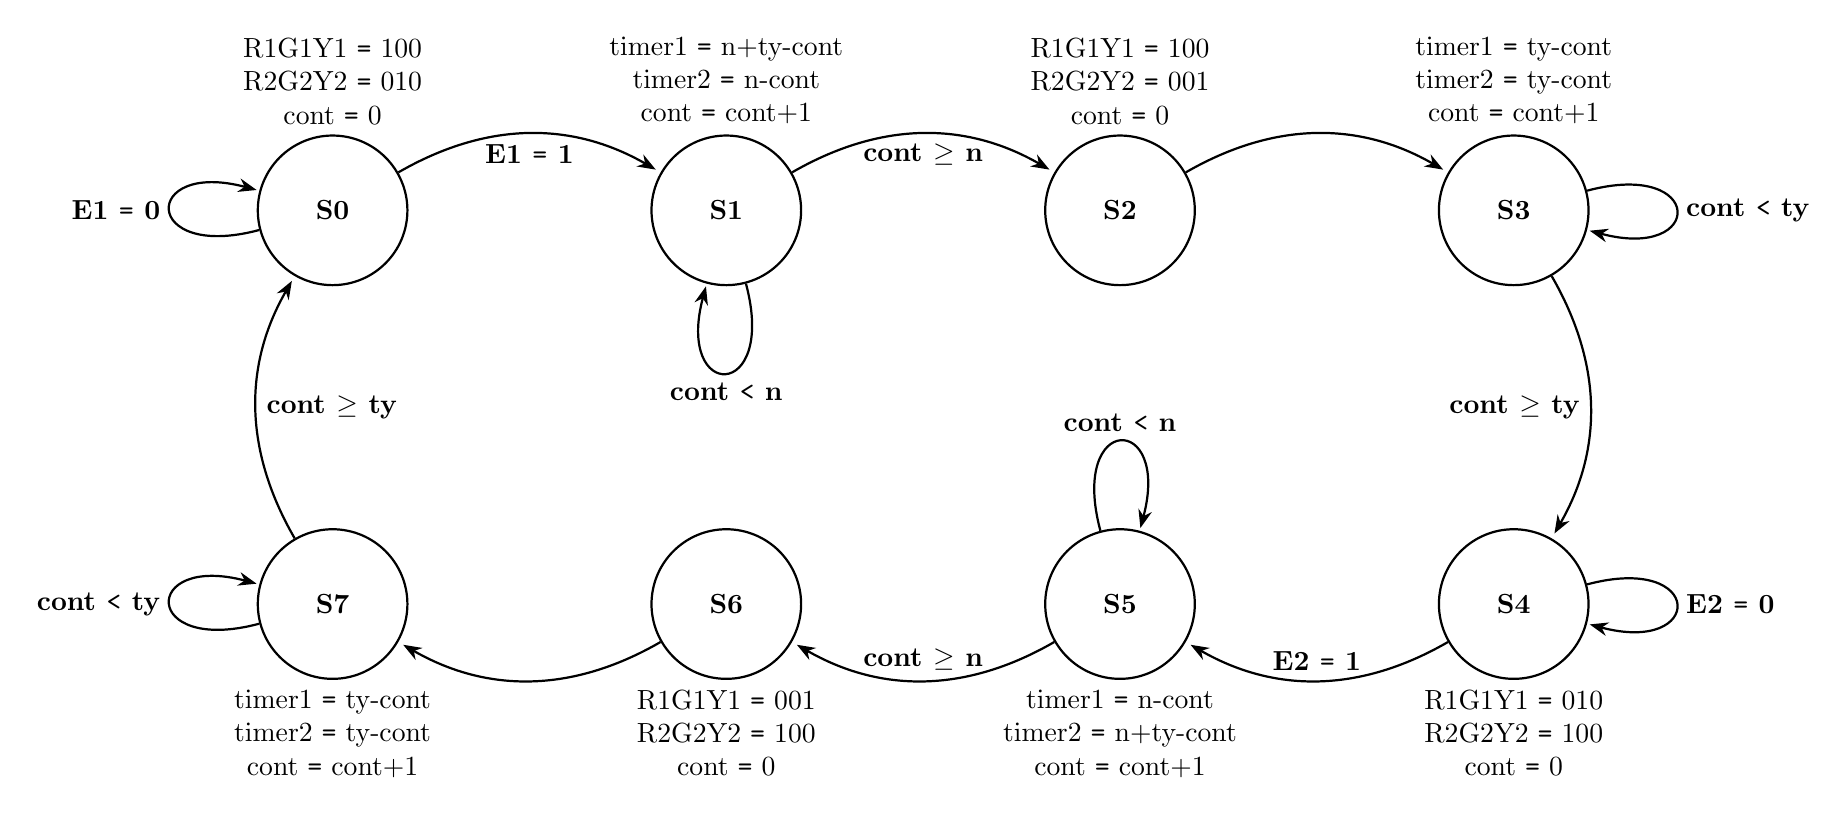
\begin{tikzpicture}[->,>=Stealth,shorten >=2pt,auto,node distance=5cm,thick]
  \tikzstyle{every state}=[fill=white,draw=black,text=black]

  \node[state, minimum width=1.9cm, minimum height=1.9cm] (S0) {\textbf{S0}};
  \node[state, minimum width=1.9cm, minimum height=1.9cm] (S1) [right of=S0] {\textbf{S1}};
  \node[state, minimum width=1.9cm, minimum height=1.9cm] (S2) [right of=S1] {\textbf{S2}};
  \node[state, minimum width=1.9cm, minimum height=1.9cm] (S3) [right of=S2] {\textbf{S3}};
  \node[state, minimum width=1.9cm, minimum height=1.9cm] (S4) [below of=S3] {\textbf{S4}};
  \node[state, minimum width=1.9cm, minimum height=1.9cm] (S5) [left of=S4] {\textbf{S5}};
  \node[state, minimum width=1.9cm, minimum height=1.9cm] (S6) [left of=S5] {\textbf{S6}};
  \node[state, minimum width=1.9cm, minimum height=1.9cm] (S7) [left of=S6] {\textbf{S7}};

  \path (S0) edge [bend left] node[midway, below][font=\bfseries] {E1 \texttt{=} 1} (S1)
        (S1) edge [bend left] node[midway, below][font=\bfseries] {cont $\geq$ n} (S2)
        (S2) edge [bend left] node[midway, below][font=\bfseries] {} (S3)
        (S3) edge [bend left] node[midway, left][font=\bfseries] {cont $\geq$ ty} (S4)
        (S4) edge [bend left] node[midway, above][font=\bfseries] {E2 \texttt{=} 1} (S5)
        (S5) edge [bend left] node[midway, above][font=\bfseries] {cont $\geq$ n} (S6)
        (S6) edge [bend left] node[midway, above][font=\bfseries] {} (S7)
        (S7) edge [bend left] node[midway, right][font=\bfseries] {cont $\geq$ ty} (S0);
  \path (S0) edge[loop left] node[font=\bfseries] {E1 \texttt{=} 0} (S0);
  \path (S1) edge[loop below] node[font=\bfseries] {cont \texttt{<} n} (S1);
  \path (S3) edge[loop right] node[font=\bfseries] {cont \texttt{<} ty} (S3);
  \path (S4) edge[loop right] node[font=\bfseries] {E2 \texttt{=} 0} (S4);
  \path (S5) edge[loop above] node[font=\bfseries] {cont \texttt{<} n} (S5);
  \path (S7) edge[loop left] node[font=\bfseries] {cont \texttt{<} ty} (S7);

  \node[align=center, text width=5cm, above] at (S0.north) {R1G1Y1 \texttt{=} 100\\R2G2Y2 \texttt{=} 010\\cont \texttt{=} 0};
  \node[align=center, text width=5cm,above] at (S1.north) {timer1 \texttt{=} n+ty-cont\\timer2 \texttt{=} n-cont\\cont \texttt{=} cont+1};
  \node[align=center, text width=5cm,above] at (S2.north) {R1G1Y1 \texttt{=} 100\\R2G2Y2 \texttt{=} 001\\cont \texttt{=} 0};
  \node[align=center, text width=5cm,above] at (S3.north) {timer1 \texttt{=} ty-cont\\timer2 \texttt{=} ty-cont\\cont \texttt{=} cont+1};
  \node[align=center, text width=5cm,below] at (S4.south) {R1G1Y1 \texttt{=} 010\\R2G2Y2 \texttt{=} 100\\cont \texttt{=} 0};
  \node[align=center, text width=5cm,below] at (S5.south) {timer1 \texttt{=} n-cont\\timer2 \texttt{=} n+ty-cont\\cont \texttt{=} cont+1};
  \node[align=center, text width=5cm,below] at (S6.south) {R1G1Y1 \texttt{=} 001\\R2G2Y2 \texttt{=} 100\\cont \texttt{=} 0};
  \node[align=center, text width=5cm,below] at (S7.south) {timer1 \texttt{=} ty-cont\\timer2 \texttt{=} ty-cont\\cont \texttt{=} cont+1};
\end{tikzpicture}
\end{landscape}
\end{document}